\chapter{Coherence walls and the coherence optimum}\label{ch:walls}
% Numbers: docs/book/figscripts/fig_p3_devices_g3.py (illustrative a/b = 1, 3, 10).

\section{Three components of a gate error}

The qubit gauge (Section~\ref{sec:devicegauges}) splits a superconducting two-qubit error into three parts:
\begin{equation}
 p_{2Q}=p_{\mathrm{coh}}+p_{\mathrm{mat}}+p_{\mathrm{ctrl}} .
 \label{eq:pdecomp}
\end{equation}
Here $p_{\mathrm{coh}}$ is the error from finite $T_1$ and $T_2$ over the gate time. For a gate of duration $t_g$,
$p_{\mathrm{coh}}\approx t_g/T_1+t_g/T_\phi$ up to state-averaging factors~\cite{Abad2022} \derived. The second term,
$p_{\mathrm{mat}}$, is the error contributed by the two-level systems (TLS) of the device's surfaces and
interfaces. The gauge takes it to grow as $T_1$ approaches the ceiling $T_{1,\mathrm{free}}$ that these TLS allow.
The third, $p_{\mathrm{ctrl}}$, is the control and crosstalk overhead. Only the first term follows from standard theory.
The split between the second and the third is a model \conjecture.

\section{A coherence optimum}

The simplest forms with these properties are $p_{\mathrm{coh}}=a/T_1$ and $p_{\mathrm{mat}}=b/(T_{1,\mathrm{free}}-T_1)$,
with $a$ and $b$ constants of the device. Their sum is smallest where $a/T_1^2=b/(T_{1,\mathrm{free}}-T_1)^2$, that is at
\begin{equation}
 \frac{T_1^*}{T_{1,\mathrm{free}}}=\frac{r}{1+r},\qquad r=\sqrt{a/b}.
 \label{eq:t1star}
\end{equation}
\derived\ (within the model). Beyond $T_1^*$ a device on the same material that gains $T_1$ loses more to the material
term than it gains in coherence. Where the optimum sits is set by the device constants $a$ and $b$, so it is a property of each
device, not a universal number (Figure~\ref{fig:coherence_optimum}). The model itself is a \conjecture: no physical mechanism has been identified by
which a rising $T_1$ would raise $p_{\mathrm{mat}}$. In standard theory TLS loss lowers $T_1$~\cite{Martinis2005,Muller2019};
the material term can rise while $T_1$ rises only if a second channel, such as crosstalk through a denser coupler
graph, changes at the same time.

\begin{figure}[htbp]\centering
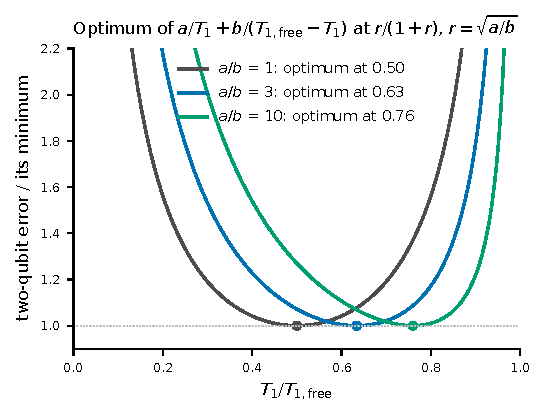
\includegraphics[width=0.62\textwidth]{figures/part5/fig_p3_coherence_optimum.pdf}
\caption{The model $p=a/T_1+b/(T_{1,\rm free}-T_1)$, each curve divided by its own minimum, for the illustrative ratios $a/b=1$, 3 and 10.
The optimum sits at $T_1^*/T_{1,\rm free}=r/(1+r)$ with $r=\sqrt{a/b}$: 0.50, 0.63 and 0.76.
\derived\ (form) \calc\ (values)}\label{fig:coherence_optimum}
\end{figure}

\section{Where the ceiling comes from}

Most TLS loss in present transmons sits in the amorphous oxides at the metal--air, metal--substrate and substrate--air
interfaces and on the junction leads~\cite{Wang2015TLS,Lisenfeld2019,Lisenfeld2025}. The Josephson junction itself is
Al/AlO$_x$/Al whatever the base metal of the pads and wiring. Tantalum base layers raised $T_1$ to 0.3--0.5~ms~\cite{Place2021,Wang2022Ta}
\observed. Their native oxide is amorphous Ta$_2$O$_5$ with suboxides near the metal, and its loss is lower than that of
niobium oxides~\cite{Crowley2023}. Electron microscopy and electron energy-loss spectroscopy of the two native oxides find that the niobium surface oxide passes gradually
from Nb$_2$O$_5$ through NbO$_2$ and NbO to the metal, and that the tantalum surface oxide has fewer suboxides than the niobium
oxide~\cite{Oh2024} \observed. Encapsulating niobium so that its native oxide does not form gave $T_1$ two to five times longer than
baseline niobium devices, and with a tantalum cap median lifetimes above 300~$\mu$s and maximum values up to 600~$\mu$s; the comparison
across capping materials showed the detrimental effect of the niobium oxides against the native oxides of tantalum, aluminum and
titanium nitride~\cite{Bal2024} \observed. On aluminum, growing the film thicker than 300~nm leaves fewer oxide-bearing grain
boundaries near the substrate--metal interface and lowers the TLS loss; aluminum-on-silicon transmons made this way reached
time-averaged $T_1$ up to 270~$\mu$s and a highest observed value of 501~$\mu$s~\cite{Biznarova2024} \observed. The base metal also
changes the quasiparticle channel. The coherence gain of tantalum comes primarily from reduced dielectric loss at the metal--air
interface, and with infrared filters installed, niobium and tantalum offset-charge-sensitive qubits showed tunneling rates of 100~Hz
and 300~Hz respectively, with both infrared channels significant for tantalum but not for niobium~\cite{Kerschbaum2026} \observed. A
change of material can move the dielectric ceiling and the quasiparticle floor in different directions, and both are measured on the
device \interp. The 105-qubit aluminum processor of Ref.~\cite{GoogleWillow2025} has a mean
$T_1=68~\mu$s and $T_{2,\mathrm{CPMG}}=89~\mu$s \observed. The ceiling $T_{1,\mathrm{free}}$ of a given material and geometry is a
quantity to be measured, from TLS spectroscopy and from $T_1$ on devices that differ only in participation ratio \openprob.

\section{The test}

\prediction\ On one material and at fixed connectivity, a device whose $T_1$ lies beyond its own optimum,
Eq.~\eqref{eq:t1star}, has a higher two-qubit error than a device near the optimum. The model fails if, at fixed
topology and material, $p_{2Q}$ keeps falling as $T_1$ rises through $T_1^*$. The test needs $T_1$, $T_\phi$, the gate
time and the isolated two-qubit error measured on the same devices and published together. A layered-circuit benchmark
such as the error per layered gate~\cite{McKay2023} includes simultaneous operation, single-qubit errors and crosstalk;
it is a different quantity and cannot stand in for an isolated two-qubit error.

\openprob\ No published pair of devices on one material and one coupler topology yet makes this comparison. The
constants $a$ and $b$ of Eq.~\eqref{eq:t1star} have not been measured on any device, so the location of the optimum is
not yet known for any processor. A laboratory that publishes the four quantities together on two devices of one material can locate it.

\section{The same optimum in other classes}\label{sec:walls_other}

The structure of Eq.~\eqref{eq:t1star}, a dominant error that falls as one quantity improves and a secondary one that grows with it, is
not special to superconductors \conjecture. In a laser-gate ion trap the two-qubit error can be written
\begin{equation}
 p_{2Q}=\frac{A}{P}+BP+p_{\mathrm{ctrl}},\qquad B=\eta^2\Bigl(\frac{\pi}{2}\Bigr)^2\frac{\Gamma_{\mathrm{heat}}\,t_g}{P_{\mathrm{ref}}},
 \label{eq:walls_mhi}
\end{equation}
with $P$ the effective laser drive, $A/P$ the laser-noise part, $BP$ the motional-heating part, $\eta$ the Lamb--Dicke parameter and
$\Gamma_{\mathrm{heat}}$ the heating rate in quanta per second. The minimum lies at $P^*=\sqrt{A/B}$, where the two parts are equal and
their sum is $2\sqrt{AB}$ \derived\ (within the model). For $\eta=0.07$ the prefactor $\eta^2(\pi/2)^2$ is $0.0121$ \calc. Sympathetic
cooling with a co-trapped species lowers $\Gamma_{\mathrm{heat}}$ and moves $P^*$ outward, the ion-trap counterpart of changing the base
metal of a superconducting chip \interp. The constants $A$ and $B$ have not been measured on one system, and the heating rates and gate
times that would place a given processor on Eq.~\eqref{eq:walls_mhi} are \openprob. One system measured with and without sympathetic
cooling, at fixed drive, shows the shift of $P^*$ directly.

\noindent One heating-rate measurement is available for a trap of this kind: background heating of $29\pm4$ quanta/s for the center-of-mass mode and
$3.0\pm0.5$ quanta/s for the stretch mode of a $^{138}$Ba$^+$--$^{171}$Yb$^+$ crystal in an X-junction surface-electrode trap~\cite{Burton2023}
\observed. It is a rate for that trap and crystal; it does not by itself give $B$ for a processor, which also needs that processor's Lamb--Dicke
parameter, gate time and drive. The same structure appears in a neutral-atom Rydberg gate, where the decay part falls with the drive and the
blockade-leakage and scattering parts rise with it, $p(\Omega)=a/\Omega+b\Omega^2+p_{\rm ctrl}$, with its minimum at $\Omega^*=(a/2b)^{1/3}$
\derived\ (within the model; Chapter~\ref{ch:qplatforms}).

\paragraph{Qubit count.} A published two-qubit error is measured on one pair with its neighbors idle. Counting each coupler as one more
crosstalk path, the error of a gate inside a full circuit can be written $p_{\mathrm{eff}}=1-(1-p_{2Q})^{1+\alpha C(N)}\approx
p_{2Q}\,(1+\alpha C(N))$, with $C(N)$ the couplers per qubit and $\alpha$ a crosstalk coefficient \conjecture; the linear form differs from the exact one
by at most $4\times10^{-6}$ in absolute terms (about $10^{-3}$ relative) for $p_{2Q}\le2\times10^{-3}$ and $\alpha C\le1$ \calc. On a fixed lattice $C$ stays near constant as qubits
are added. On the heavy-hexagon lattice, laid out for superconducting qubits to limit frequency collisions and crosstalk, qubits have degree two
or three~\cite{Chamberland2020PRX} \observed. In a reconfigurable neutral-atom array the atoms are moved between zones, which gives
arbitrary connectivity~\cite{Bluvstein2024} \observed; there the effective $C$ is set by the movement schedule rather than by a fixed
lattice \interp. In a shuttling (QCCD) trap the effective connectivity grows slowly with $N$; for logarithmic growth, doubling the qubit count from
about 100 to about 200 raises it by $\ln200/\ln100=1.15$ \calc. That $\alpha$ jumps when a superconducting device passes its own $T_1^*$ is a
\conjecture: no published pair of devices on one material and one coupler topology yet separates it from the change of topology itself.

\paragraph{The cryostat as part of the surface.} The qubit count also has a thermal side. Every control line connects room-temperature
electronics to the processor and loads the refrigerator, passively by heat conduction and actively by the dissipation of control signals
in its cables and attenuators~\cite{Krinner2019} \observed. The dilution refrigerator of that study offers about 13~$\mu$W of
cooling at 20~mK on its mixing chamber at its standard flow, and up to about 19~$\mu$W at a raised flow; a cabling scheme engineered for that budget supports 50 qubits at 14~mK and,
disregarding space, at least 150~\cite{Krinner2019} \observed. Beyond some count, wiring heat load, crosstalk and cooling power together
set an integration ceiling for each chip and cryostat, a system-level limit separate from the material ceiling of one junction \interp.

Any device lab can test this directly: two chips on the same material and coupler layout, one pushed past the optimum, and the two-qubit error
measured on both.
